\documentclass[tikz]{standalone}
\usepackage{amsmath,amssymb,multirow}
\usetikzlibrary{shapes.misc, positioning,automata,arrows,calc,fit}
\tikzset{VertexStyle/.style = {draw,circle,thick,
		minimum size=1cm,
		font=\Large\bfseries},thick} 
\begin{document}
	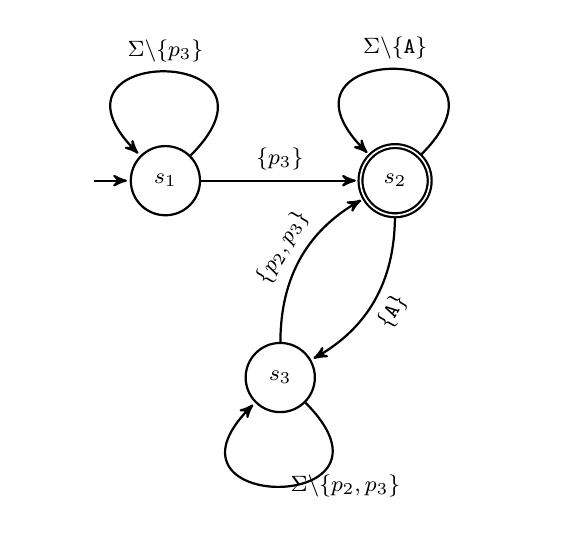
\begin{tikzpicture}[->,>=stealth',shorten >=1pt,thick,initial text=$ $,align=center,node distance=5mm,font=\footnotesize]
	\thickmuskip=0mu
	\node[state,initial] (SA) {$s_1$};
	\path (SA) edge[loop] node[midway,above] (W1) {$\Sigma\backslash\{p_3\}$} (SA);
	\node[state,accepting,right =2cm of SA] (ST) {$s_2$};
	\path (ST) edge[loop] node[midway,above] (W2) {$\Sigma\backslash\{\texttt{A}\}$} (ST);
	\draw[->] (SA) -- (ST) node[midway,above] {$ \{p_3\}$};
	\node[state] (bot) at ($(SA)!0.5!(ST)-(0,2.5)$) {$s_3$};
	\draw[->] (ST) edge [bend left] node[midway,below,sloped] {$\{\texttt{A}\}$}  (bot)  ; 
	\draw[->] (bot) 
	edge [bend left] node[midway,above,sloped] {$\{p_2,p_3\}$} (ST)  ;
	\draw (bot) to [in=225,out=315,looseness=8] node[above,right] (W3) {$\Sigma\backslash\{p_2,p_3\}$} (bot);
	\end{tikzpicture}
\end{document}